\documentclass{beamer}
\usepackage{geometry}
\usepackage[english]{babel}
\usepackage[utf8]{inputenc}
\usepackage{amsmath}
\usepackage{amsfonts}
\usepackage{amssymb}
\usepackage{tikz}
\usetikzlibrary{quotes, angles}
\usepackage{graphicx}

\usepackage{multicol}
%\usepackage{pgfplots}
%\pgfplotsset{width=10cm,compat=1.9}
%\usepackage{pgfplotstable}

\usepackage{fancyhdr}
\pagestyle{fancy}
\setlength{\headheight}{12pt}%doesn't seem to fix warning
\fancyhf{}

%\rhead{\small{24 February 2020}}
\lhead{\small{BECA / Dr. Huson / Unit 11: Analytic geometry and trigonometry}}

\renewcommand{\headrulewidth}{0pt}

\title{Mathematics Class Slides}
\subtitle{Bronx Early College Academy}
\author{Chris Huson}
\date{23 March 2020}

\begin{document}
\frame{\titlepage}
\section[Outline]{}
\frame{\tableofcontents}

\section{11.1 Deltamath point-slope practice, Tuesday 24 March} 
\frame
{
  \frametitle{GQ: How do we write a linear equation given a point and slope?}
  \framesubtitle{CCSS: HSG.CO.B6-8 Understand congruence in terms of rigid motions \hfill \alert{11.1 Monday 23 March}}

  \begin{block}{Do Now: Welcome to Beca Online!}
    \begin{itemize}
      \item Complete the attendance question in Google Classroom
      \item Write in your notebook my new email, chuson@beca324.org
      \item Complete the G-Classroom ``Do Now" questions
    \end{itemize}

    \end{block}
    BECA Online expectations \\[0.25cm]
    Lesson: \\
    Point-slope form of linear equations \\
    Khan Academy video \& Deltamath practice problems  \\
    Homework: Complete Deltamath practice, due by 10:00pm
}

\section{11.2 Circle equations review, Thursday 26 March} 
\frame
{
  \frametitle{GQ: How do we define a circle with an equation?}
  \framesubtitle{CCSS: HSG.GPE.A1 Geometry \& equations of conics \hfill \alert{11.2 Thursday 26 March}}

  \begin{block}{Do Now: Point-slope assessment; answer by Zoom private message}
    \begin{enumerate}
      \item What is the slope of $y=\frac{3}{2}x+5$?
      \item Find the $y$-intercept of $4x-y=7$
      \item Identify a point on the line $y-3=\frac{1}{2}(x+1)$ as an ordered pair
      \item Identify a point on the line $y=\frac{1}{2}x+6$ as an ordered pair
      \item Find the equation of the line with slope 2 through $(-4,9)$
    \end{enumerate}

    \end{block}
    Lesson: Finding the center and radius of a circle given its equation \\
    Video, Desmos discussion; Deltamath classwork ``Circle Equations''  \\
    Extra credit: Deltamath ``System of Equations of Circle/Line (L1)" \\[0.25cm]
    Daily practice: Khan Academy triangle \& parallelogram areas
}

\frame
{
  \frametitle{GQ: How do we define a circle with an equation?}
  \framesubtitle{CCSS: HSG.GPE.A1 Geometry \& equations of conics \hfill \alert{11.2 Thursday 26 March}}

  \begin{block}{Do Now: Point-slope assessment; \alert{Answers}}
    \begin{enumerate}
      \item What is the slope of $y=\alert{\frac{3}{2}}x+5$? \alert{Answer $\frac{3}{2}$}
      \item Find the $y$-intercept of $4x-y=7$ \alert{Answer $-7$}
      \item Identify a point on the line $y \alert{-3}=\frac{1}{2}(x \alert{+1})$ as an ordered pair \\
      \hspace{1cm} \alert{Answer $(-1,3)$}
      \item Identify a point on the line $y=\frac{1}{2}x \alert{+6}$ as an ordered pair \\
      \hspace{1cm} \alert{$(0,6)$, the $y$-intercept; others: $(2,7)$, $(3,8)$, etc}
      \item Find the equation of the line with slope 2 through $(-4,9)$ \\
      \hspace{1cm} \alert{Answer:} $y \alert{-9}=\alert{2}(x \alert{+4})$
    \end{enumerate}
    \end{block}
}

\section{11.3 Circle area and circumference, Tuesday 31 March} 
\frame
{
  \frametitle{GQ: How do we calculate area \& circumference of circles?}
  \framesubtitle{CCSS: HSG.GPE.A1 Geometry \& equations of conics \hfill \alert{11.3 Tuesday 31 March}}

  \begin{block}{Do Now: Simple area and perimeter. (answer in G-Classroom)}
    \begin{enumerate}
      \item Find the area of the triangle.
      \item Find the area and perimeter of the semi-circle.
    \end{enumerate}
    \end{block}
    \begin{center}
      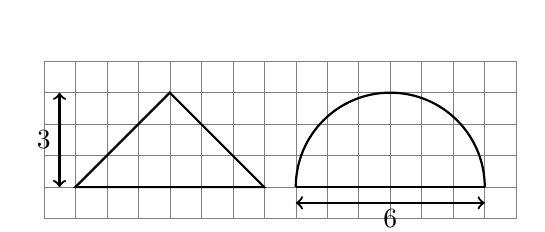
\begin{tikzpicture}[scale=.4]
        \draw [help lines] (-1,-1) grid (14,4);
        %\draw [thick, ->] (-2.2,0) -- (8.4,0) node [below right] {$x$};
        %\draw [thick, ->] (0,-1.2)--(0,7.4) node [left] {$y$};
        \draw [thick] (7,0)--(13,0);
        \draw [thick] (0,0)--(3,3)--(6,0)--cycle;
        \draw [thick] (13,0) arc (0:180:3);
        %\draw [thick] (0,0) arc (-110:-70:8.9);
        %\draw [thick] (0,8) arc (-110:-70:8.9);
        %\draw [dashed] (0,8) arc (110:70:8.9);
        \draw [thick, <->] (-0.5,0)--(-0.5,3);
        \node at (-1,1.5){$3$};
        \draw [thick, <->] (7,-0.5)--(13,-0.5);
        \node at (10,-1){$6$};
      \end{tikzpicture}
    \end{center}
    Lesson: \\
    \; Simple areas, compound shapes, ``negative'' space (subtracting) \\ 
    Classwork: Deltamath (extra homework problems)\\ 
    Daily math work: Khan Academy circle practice
}

\frame
{
  \frametitle{Do Now: Solutions of area and perimeter of simple shapes}
  \begin{multicols}{2}
      Triangle: $A=\frac{1}{2}bh$ \\[0.25cm]
      \begin{flushright}
      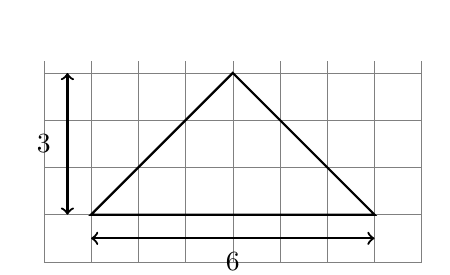
\begin{tikzpicture}[scale=.6]
        \draw [help lines] (-1,-1) grid (7,3.25);
        \draw [thick] (0,0)--(3,3)--(6,0)--cycle;
        \draw [thick, <->] (-0.5,0)--(-0.5,3);
        \node at (-1,1.5){$3$};
        \draw [thick, <->] (0,-0.5)--(6,-0.5);
        \node at (3,-1){$6$};
      \end{tikzpicture}
    \end{flushright}
    \end{multicols}
    \begin{multicols}{2}
      Circle:  \\[0.25cm] $A=\pi r^2$ \qquad $C=\pi D = 2 \pi r$
      \begin{flushright}
      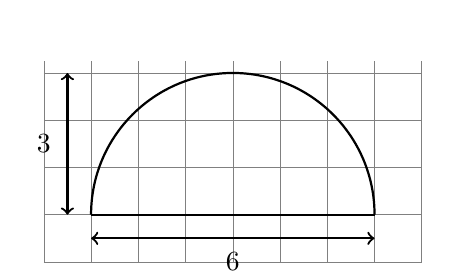
\begin{tikzpicture}[scale=.6]
        \draw [help lines] (-1,-1) grid (7,3.25);
        \draw [thick] (0,0)--(6,0);
        \draw [thick] (6,0) arc (0:180:3);
        \draw [thick, <->] (-0.5,0)--(-0.5,3);
        \node at (-1,1.5){$3$};
        \draw [thick, <->] (0,-0.5)--(6,-0.5);
        \node at (3,-1){$6$};
      \end{tikzpicture}
    \end{flushright}
    \end{multicols} \vspace{2cm}
}

\frame
{
  \frametitle{Compound shapes, ``negative space'' or subtracting areas}
  \begin{multicols}{2}
      Find the area of the shaded region.
      \begin{flushright}
      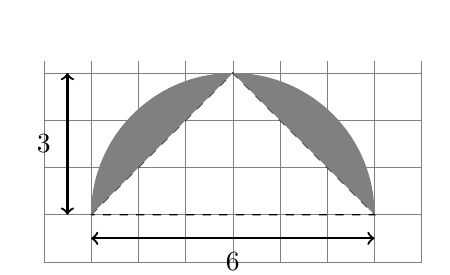
\begin{tikzpicture}[scale=.6]
        \draw [help lines] (-1,-1) grid (7,3.25);
        %\draw [dashed] (0,0)--(6,0);
        \draw [dashed] (0,0)--(3,3)--(6,0)--cycle;
        %\draw [thick] (6,0) arc (0:180:3);
        \fill [gray] (6,0) arc (0:90:3)--(6,0);
        \fill [gray] (0,0) arc (180:90:3)--(0,0);
        \draw [thick, <->] (-0.5,0)--(-0.5,3);
        \node at (-1,1.5){$3$};
        \draw [thick, <->] (0,-0.5)--(6,-0.5);
        \node at (3,-1){$6$};
      \end{tikzpicture}
    \end{flushright}
    \end{multicols} \vspace{1cm}
    \begin{multicols}{2}
      Challenge: Find the area of the shaded regions.
      \begin{flushright}
      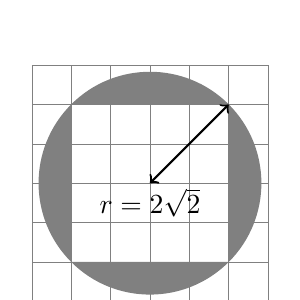
\begin{tikzpicture}[scale=.5]
        \draw [help lines] (-3,-3) grid (3,3);
        %\draw [dashed] (0,0)--(6,0);
        \draw [thick, <->] (0,0)--(45:2.83);
        %\draw [thick] (6,0) arc (0:180:3);
        \fill [gray] (-45:2.83) arc (-45:45:2.83)--cycle;
        \fill [gray] (45:2.83) arc (45:135:2.83)--cycle;
        \fill [gray] (-45:2.83) arc (-45:-135:2.83)--cycle;
        \fill [gray] (-135:2.83) arc (-135:-225:2.83)--cycle;
        \node at (0,-0.5){$r=2 \sqrt{2}$};
      \end{tikzpicture}
    \end{flushright}
    \end{multicols} \vspace{2cm}
}


\frame
{
  \frametitle{Find the area of the triangle}

      \begin{flushright}
      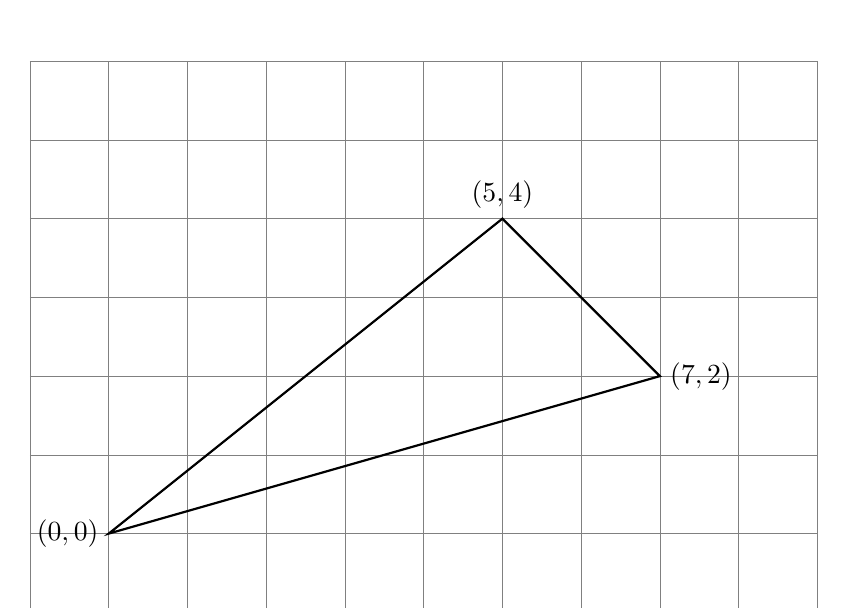
\begin{tikzpicture}[scale=1.0]
        \draw [help lines] (-1,-1) grid (9,6);
        \draw [thick] (0,0)node[left]{$(0,0)$}--
        (5,4)node[above]{$(5,4)$}--
        (7,2)node[right]{$(7,2)$}--cycle;
        %\draw [thick, <->] (-0.5,0)--(-0.5,3);
        %\node at (-1,1.5){$3$};
        %\draw [thick, <->] (0,-0.5)--(6,-0.5);
        %\node at (3,-1){$6$};
      \end{tikzpicture}
    \end{flushright}
    
}

\end{document}

